\documentclass{standalone}
\usepackage{tikz}
\usetikzlibrary{matrix, positioning, shapes, arrows, calc}

\tikzset{>=latex}

\begin{document}


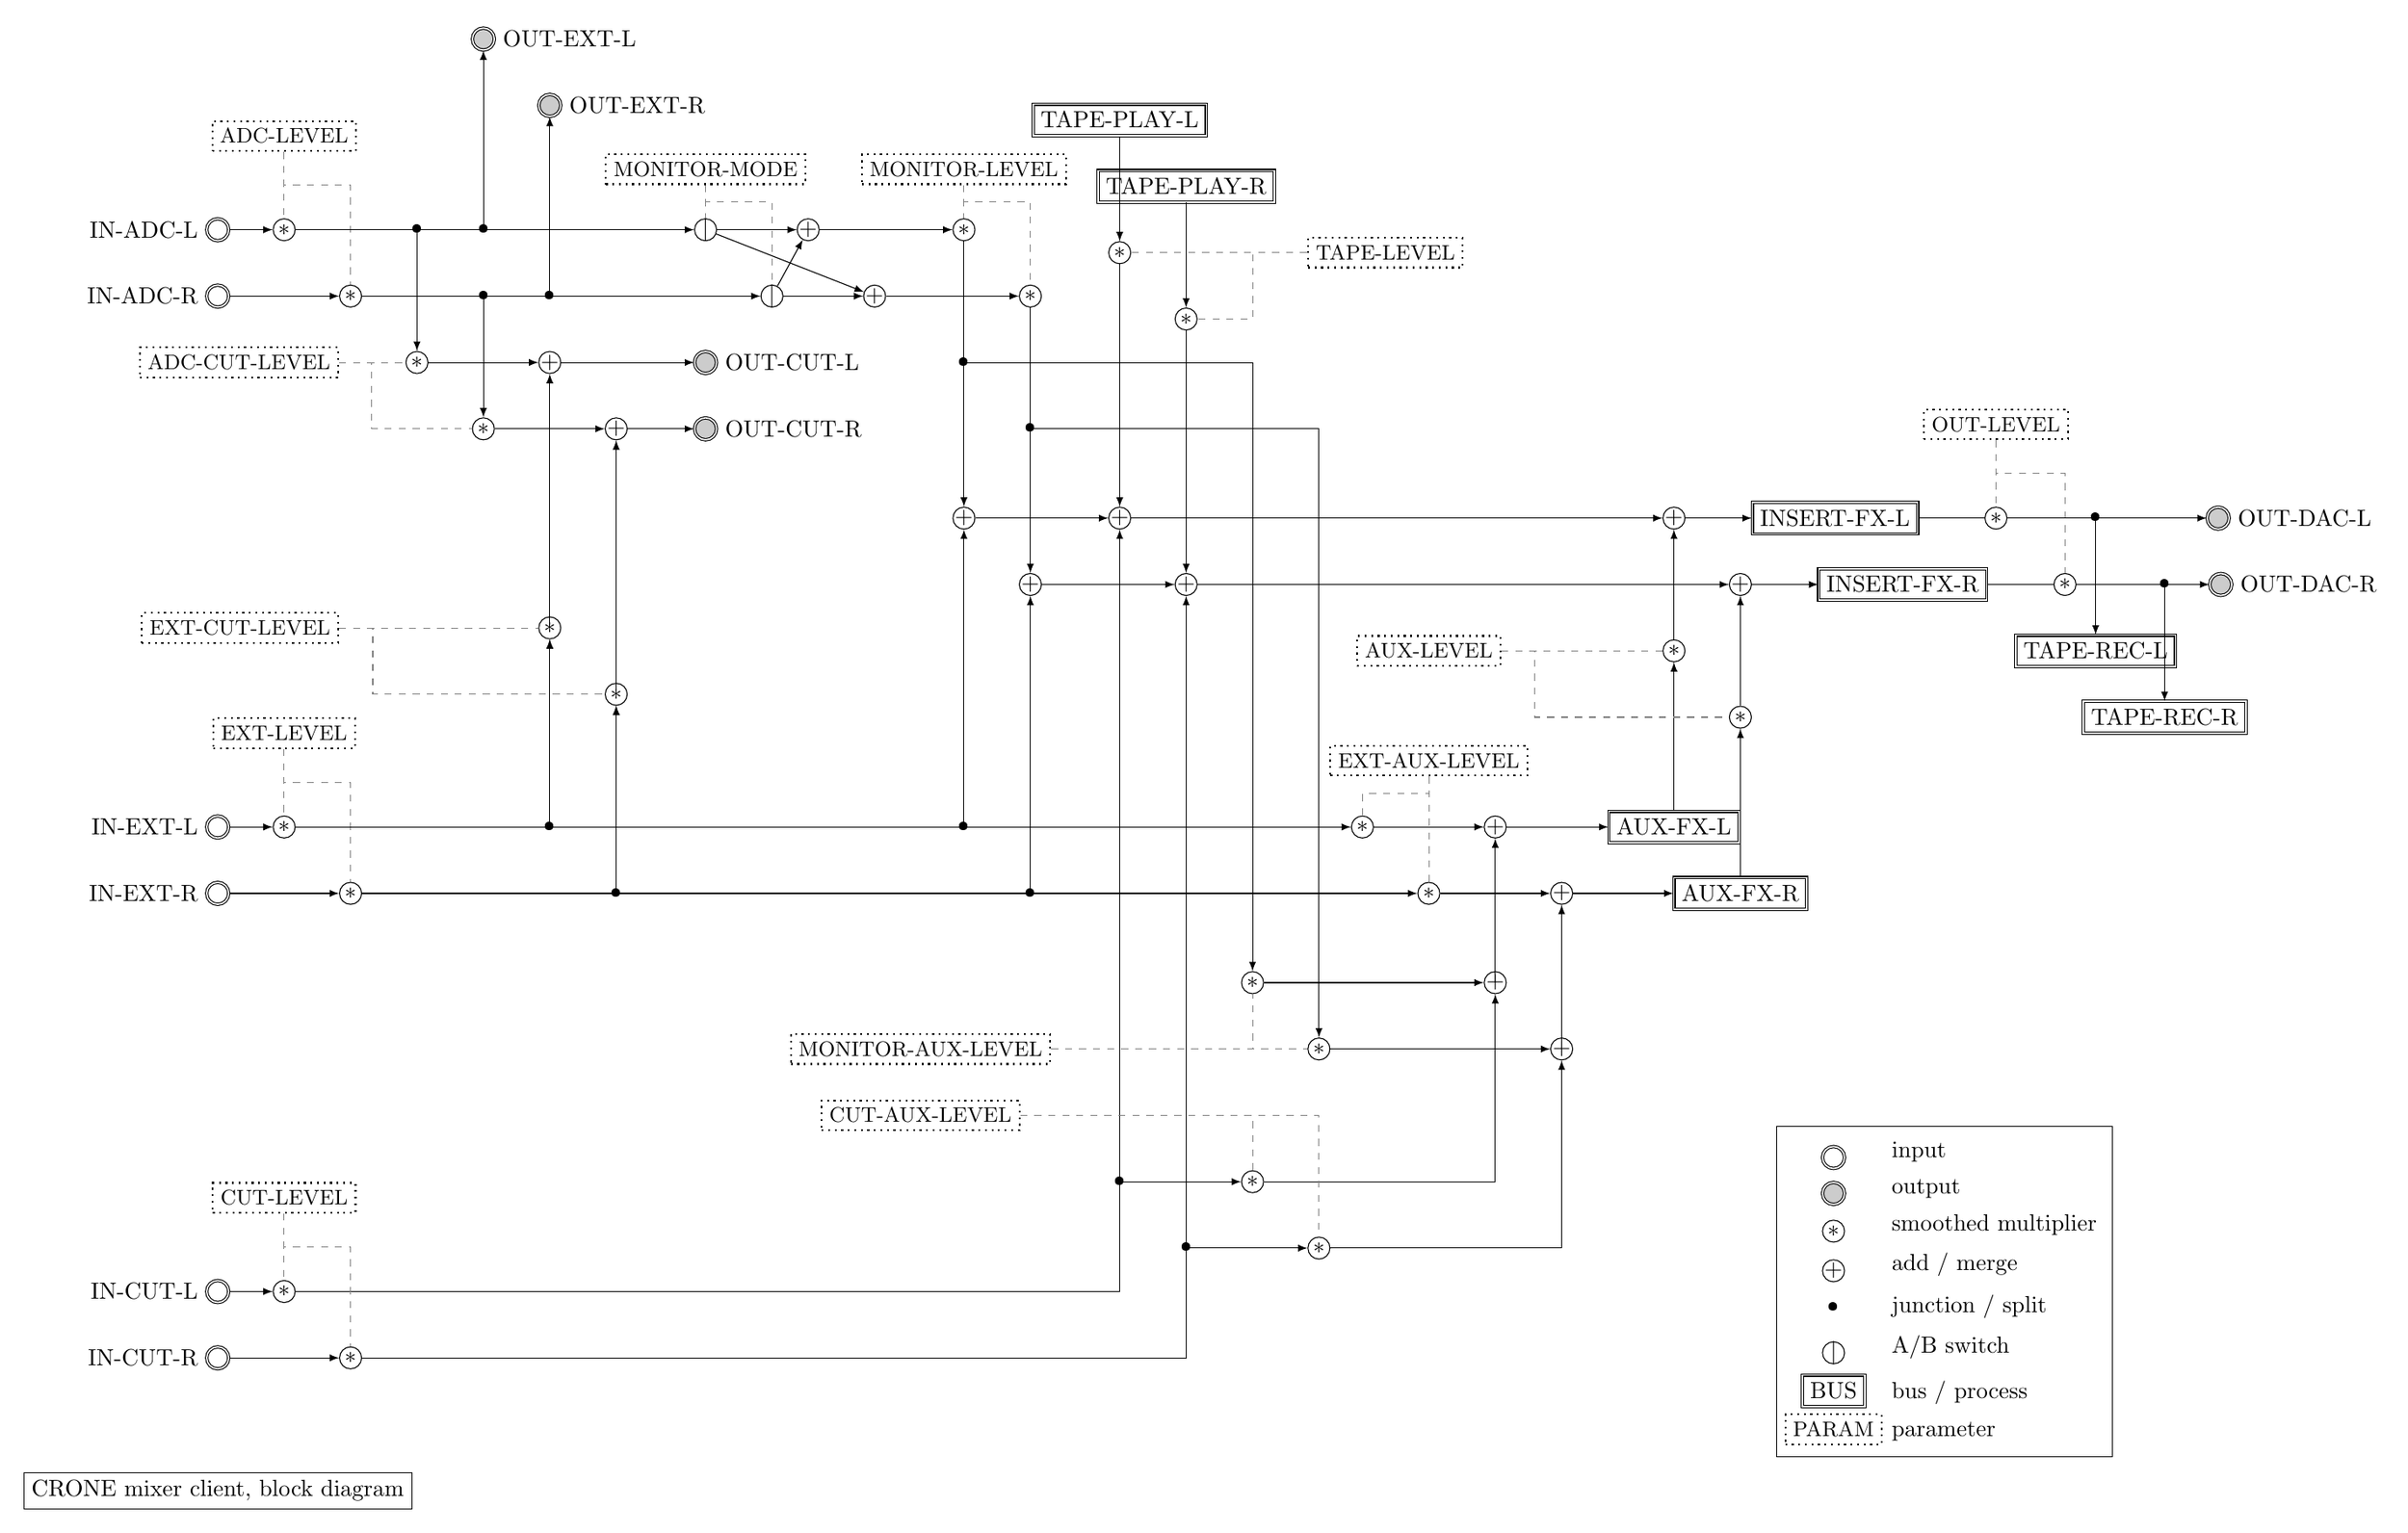
\begin{tikzpicture}

\tikzstyle{input}=[draw=black, circle, double, minimum size=1]
\tikzstyle{output}=[draw=black, circle, double, minimum size=1, fill=gray!40]
\tikzstyle{mul}=[draw=black, circle, minimum size=1, label=center:$\ast$]
\tikzstyle{add}=[draw=black, circle, minimum size=1, label=center:$+$]
\tikzstyle{or}=[draw=black, circle, minimum size=1, label=center:$|$]
\tikzstyle{param}=[draw=black, rectangle, dotted, thick]
\tikzstyle{bus}=[draw=black, rectangle, double]

\node [draw] at (0, -2) {CRONE mixer client, block diagram};

%%%%%%%%%%%%%%%%%%%%%%%%%%%%
% input nodes
\node [input, label=left:IN-ADC-L] (in-adc-l) at (0, 17) {};
\node [input, label=left:IN-ADC-R] (in-adc-r) at (0, 16){};
\node [input, label=left:IN-EXT-L] (in-ext-l) at (0, 8) {};
\node [input, label=left:IN-EXT-R] (in-ext-r) at (0, 7) {};
\node [input, label=left:IN-CUT-L] (in-cut-l) at (0, 1) {};
\node [input, label=left:IN-CUT-R] (in-cut-r) at (0, 0) {};

%%%%%%%%%%%%%%%%%%
%% ADC section

% ADC levels
\node [mul] (adc-mul-l) at ($(in-adc-l)+(1,0)$) {};
\node [mul] (adc-mul-r) at ($(in-adc-r)+(2,0)$) {};
\draw [->] (in-adc-l) -- (adc-mul-l);
\draw [->] (in-adc-r) -- (adc-mul-r);
\node [param, above = 1 of adc-mul-l] (adc-level) {\small{ADC-LEVEL}};
\draw [gray, dashed] (adc-level.south) -- ++(0, -0.5) -| (adc-mul-l);
\draw [gray, dashed] (adc-level.south) -| ++(0, -0.5) -| (adc-mul-r);

% ADC to EXT
\node (adc-l-ext-junc) at ($(adc-mul-l) + (3, 0)$) {\textbullet};
\node (adc-r-ext-junc) at ($(adc-mul-r) + (3, 0)$) {\textbullet};
\node [output, label=right:OUT-EXT-L, above=2.5 of adc-l-ext-junc] (out-ext-l) {}; 
\node [output, label=right:OUT-EXT-R, above=2.5 of adc-r-ext-junc] (out-ext-r) {}; 
\draw [->] (adc-l-ext-junc.center) -- (out-ext-l);
\draw [->] (adc-r-ext-junc.center) -- (out-ext-r);


% ADC to CUT
\node (adc-cut-junc-l) at ($(adc-mul-l) + (2, 0)$) {\textbullet};
\node (adc-cut-junc-r) at ($(adc-mul-r) + (2, 0)$) {\textbullet};
\node [mul] (adc-cut-mul-l) at ($(adc-cut-junc-l) - (0, 2)$) {};
\node [mul] (adc-cut-mul-r) at ($(adc-cut-junc-r) - (0, 2)$) {}; 
\node [param, left = 1 of adc-cut-mul-l] (adc-cut) {\small{ADC-CUT-LEVEL}};
\draw [->] (adc-cut-junc-l.center) -- (adc-cut-mul-l);
\draw [->] (adc-cut-junc-r.center) -- (adc-cut-mul-r);
\draw [gray, dashed] (adc-cut) -- ++(2, 0) -- (adc-cut-mul-l);
\draw [gray, dashed] (adc-cut) -- ++(2, 0) |- (adc-cut-mul-r);

%%%%%%%%%%%%%%%%%%%%%%%%%%
%% monitor section

% monitor mix
\node [or, right=6 of adc-mul-l, minimum size=0] (monitor-mix-in-l) {};
\node [or, right=6 of adc-mul-r, minimum size=0] (monitor-mix-in-r) {};
\node [add, right=1.2 of monitor-mix-in-l] (monitor-mix-out-l) {};
\node [add, right=1.2 of monitor-mix-in-r] (monitor-mix-out-r) {};	

\draw [->] (adc-mul-l) -- (monitor-mix-in-l);
\draw [->] (adc-mul-r) -- (monitor-mix-in-r);
\draw [->] (monitor-mix-in-l) -- (monitor-mix-out-l);
\draw [->] (monitor-mix-in-l) -- (monitor-mix-out-r);
\draw [->] (monitor-mix-in-r) -- (monitor-mix-out-l);
\draw [->] (monitor-mix-in-r) -- (monitor-mix-out-r);

\node [param, above = 0.5 of monitor-mix-in-l] (monitor-mode) {\small{MONITOR-MODE}};
\draw [gray, dashed] (monitor-mode.south) -- ++(0,-0.25) -| (monitor-mix-in-l);
\draw [gray, dashed] (monitor-mode.south) -- ++(0,-0.25) -| (monitor-mix-in-r);

% monitor level
\node [mul, right=2 of monitor-mix-out-l] (monitor-mul-l) {};
\node [mul, right=2 of monitor-mix-out-r] (monitor-mul-r) {};
\draw [->] (monitor-mix-out-l) -- (monitor-mul-l);
\draw [->] (monitor-mix-out-r) -- (monitor-mul-r);
\node [param, above = 0.5 of monitor-mul-l] (monitor-level) {\small{MONITOR-LEVEL}};
\draw [gray, dashed] (monitor-level.south) -- ++(0, -0.25) -| (monitor-mul-l);
\draw [gray, dashed] (monitor-level.south) -| ++(0, -0.25) -| (monitor-mul-r);

%%%%%%%%%%%%%%%%%%%%%%%%%%
%% insert FX, DAC
\node [add, below=4 of monitor-mul-l] (ins-in-l) {};
\node [add, below=4 of monitor-mul-r] (ins-in-r) {};
\node [add, right=2 of ins-in-l] (ins-in-2-l) {};
\node [add, right=2 of ins-in-r] (ins-in-2-r) {};
\node [add, right=8 of ins-in-2-l] (ins-in-3-l) {};
\node [add, right=8 of ins-in-2-r] (ins-in-3-r) {};

\node [bus, right =1 of ins-in-3-l] (ins-fx-l) {INSERT-FX-L};
\node [bus, right =1 of ins-in-3-r] (ins-fx-r) {INSERT-FX-R}; 
\node [mul, right =1 of ins-fx-l] (dac-mul-l) {};
\node [mul, right =1 of ins-fx-r] (dac-mul-r) {}; 
\node [output, right=3 of dac-mul-l, label=right:OUT-DAC-L] (out-dac-l){}; 
\node [output, right=2 of dac-mul-r, label=right:OUT-DAC-R] (out-dac-r){}; 

\node [param, above = 1 of dac-mul-l] (dac-level) {\small{OUT-LEVEL}};
\draw [gray, dashed] (dac-level.south) -- ++(0, -0.5) -| (dac-mul-l);
\draw [gray, dashed] (dac-level.south) -| ++(0, -0.5) -| (dac-mul-r);

\draw [->] (ins-in-l) -- (ins-in-2-l);
\draw [->] (ins-in-r) -- (ins-in-2-r);
\draw [->] (ins-in-2-l) -- (ins-in-3-l);
\draw [->] (ins-in-2-r) -- (ins-in-3-r);
\draw [->] (ins-in-3-l) -- (ins-fx-l);
\draw [->] (ins-in-3-r) -- (ins-fx-r);
\draw [->] (ins-fx-l) -- (dac-mul-l) -- (out-dac-l);
\draw [->] (ins-fx-r) -- (dac-mul-r) -- (out-dac-r);
\draw [->] (monitor-mul-l) -- (ins-in-l);
\draw [->] (monitor-mul-r) -- (ins-in-r);

%%%%%%%%%%%%%%%%%%%%%%%%
%% EXT section

% EXT level
\node [mul] (ext-mul-l) at ($(in-ext-l)+(1,0)$) {};
\node [mul] (ext-mul-r) at ($(in-ext-r)+(2,0)$) {};
\draw [->] (in-ext-l) -- (ext-mul-l);
\draw [->] (in-ext-r) -- (ext-mul-r);
\node [param, above = 1 of ext-mul-l] (ext-level) {\small{EXT-LEVEL}};
\draw [gray, dashed] (ext-level.south) -- ++(0, -0.5) -| (ext-mul-l);
\draw [gray, dashed] (ext-level.south) -| ++(0, -0.5) -| (ext-mul-r);

\draw [->] (ext-mul-l) -| (ins-in-l);
\draw [->] (ext-mul-r) -| (ins-in-r);

% EXT to CUT
\node (ext-cut-junc-l) at ($(ext-mul-l) + (4, 0)$) {\textbullet};
\node (ext-cut-junc-r) at ($(ext-mul-r) + (4, 0)$) {\textbullet};
\node [mul] (ext-cut-mul-l) at ($(ext-cut-junc-l) + (0, 3)$) {};
\node [mul] (ext-cut-mul-r) at ($(ext-cut-junc-r) + (0, 3)$) {}; 
\draw [->] (ext-cut-junc-l.center) -- (ext-cut-mul-l); 
\draw [->] (ext-cut-junc-r.center) -- (ext-cut-mul-r);
\node [param, left = 3 of ext-cut-mul-l] (ext-cut) {\small{EXT-CUT-LEVEL}};
\draw [->] (ext-cut-junc-l.center) -- (ext-cut-mul-l);
\draw [->] (ext-cut-junc-r.center) -- (ext-cut-mul-r);
\draw [gray, dashed] (ext-cut) -- ++(2, 0) -- (ext-cut-mul-l);
\draw [gray, dashed] (ext-cut) -- ++(2, 0) |- (ext-cut-mul-r);

%%%%%%%%%%%%
% CUT output
\node [add] (cut-sink-l) at ($(adc-cut-mul-l) + (2, 0)$) {};
\node [add] (cut-sink-r) at ($(adc-cut-mul-r) + (2, 0)$) {};
\draw [->] (adc-cut-mul-l) -- (cut-sink-l);
\draw [->] (adc-cut-mul-r) -- (cut-sink-r);
\draw [->] (ext-cut-mul-l) -| (cut-sink-l);
\draw [->] (ext-cut-mul-r) -| (cut-sink-r);

\node [output, label=right:OUT-CUT-L, right = 2 of cut-sink-l] (out-cut-l) {}; 
\node [output, label=right:OUT-CUT-R, right = 1 of cut-sink-r] (out-cut-r) {}; 
\draw [->] (cut-sink-l) -- (out-cut-l);
\draw [->] (cut-sink-r) -- (out-cut-r);

%%%%%%%%%%%%%
% CUT input
\node [mul] (cut-mul-l) at ($(in-cut-l) + (1, 0)$) {};
\node [mul] (cut-mul-r) at ($(in-cut-r) + (2, 0)$) {};
\draw [->] (cut-mul-l) -| (ins-in-2-l);
\draw [->] (cut-mul-r) -| (ins-in-2-r);
\node [param, above = 1 of cut-mul-l] (cut-level) {\small{CUT-LEVEL}};
\draw [gray, dashed] (cut-level.south) -- ++(0, -0.5) -| (cut-mul-l);
\draw [gray, dashed] (cut-level.south) -- ++(0, -0.5) -| (cut-mul-r);
\draw [->] (in-cut-l) -- (cut-mul-l);
\draw [->] (in-cut-r) -- (cut-mul-r);

%%%%%%%%%%%%%%%%
%% TAPE section
\node [mul] (tape-mul-l) at ($(ins-in-2-l) + (0, 4)$) {};
\node [mul] (tape-mul-r) at ($(ins-in-2-r) + (0, 4)$) {};
\draw [->] (tape-mul-l) -- (ins-in-2-l);
\draw [->] (tape-mul-r) -- (ins-in-2-r);

\node [bus] (tape-play-l) at ($(tape-mul-l) + (0, 2)$) {TAPE-PLAY-L};
\node [bus] (tape-play-r) at ($(tape-mul-r) + (0, 2)$) {TAPE-PLAY-R};
\draw [->] (tape-play-l) -- (tape-mul-l);
\draw [->] (tape-play-r) -- (tape-mul-r);

\node [param] (tape-level) at ($(tape-mul-l) + (4, 0)$) {\small{TAPE-LEVEL}};
\draw [gray, dashed] (tape-level) -- ++(-2, 0) |- (tape-mul-l);
\draw [gray, dashed] (tape-level) -- ++(-2, 0) |- (tape-mul-r);

\node (tape-rec-junc-l) at ($(dac-mul-l) + (1.5, 0)$) {\textbullet};
\node (tape-rec-junc-r) at ($(dac-mul-r) + (1.5, 0)$) {\textbullet};
\node [bus] (tape-rec-l) at ($(tape-rec-junc-l) + (0, -2)$) {TAPE-REC-L};
\node [bus] (tape-rec-r) at ($(tape-rec-junc-r) + (0, -2)$) {TAPE-REC-R};
\draw [->] (tape-rec-junc-l.center) -- (tape-rec-l);
\draw [->] (tape-rec-junc-r.center) -- (tape-rec-r);

%%%%%%%%%%%%%%%%%
%% AUX section


% bus -> AUX connections
\node (monitor-aux-junc-l) at ($(monitor-mul-l) + (0,-2)$) {\textbullet};
\node (monitor-aux-junc-r) at ($(monitor-mul-r) + (0,-2)$) {\textbullet}; 
\node [mul] (monitor-aux-mul-l) at ($(ins-in-2-l) + (2, -7)$) {};
\node [mul] (monitor-aux-mul-r) at ($(ins-in-2-r) + (2, -7)$) {};
\draw [->] (monitor-aux-junc-l.center) -| (monitor-aux-mul-l);
\draw [->] (monitor-aux-junc-r.center) -| (monitor-aux-mul-r);

\node (cut-aux-junc-l) at ($(ins-in-2-l) + (0, -10)$) {\textbullet};
\node (cut-aux-junc-r) at ($(ins-in-2-r) + (0, -10)$) {\textbullet};
\node [mul] (cut-aux-mul-l) at($(cut-aux-junc-l) + (2, 0)$) {};
\node [mul] (cut-aux-mul-r) at($(cut-aux-junc-r) + (2, 0)$) {};
\draw [->] (cut-aux-junc-l.center) -- (cut-aux-mul-l);
\draw [->] (cut-aux-junc-r.center) -- (cut-aux-mul-r);


\node (ext-aux-junc-l) at (in-ext-l -| ins-in-l) {\textbullet};
\node (ext-aux-junc-r) at (in-ext-r -| ins-in-r) {\textbullet};
\node [mul] (ext-aux-mul-l) at ($(ext-aux-junc-l) + (6, 0)$) {};
\node [mul] (ext-aux-mul-r) at ($(ext-aux-junc-r) + (6, 0)$) {};
\draw [->] (ext-aux-junc-l.center) -- (ext-aux-mul-l);
\draw [->] (ext-aux-junc-r.center) -- (ext-aux-mul-r);

\node [add] (aux-in-2-l) at ($(ext-aux-mul-l) + (2, 0)$) {};
\node [add] (aux-in-2-r) at ($(ext-aux-mul-r) + (2, 0)$) {};
\node [add] (aux-in-1-l) at (monitor-aux-mul-l -| aux-in-2-l) {};
\node [add] (aux-in-1-r) at (monitor-aux-mul-r -| aux-in-2-r) {};

\draw [->] (monitor-aux-mul-l) -- (aux-in-1-l);
\draw [->] (monitor-aux-mul-r) -- (aux-in-1-r);
\draw [->] (cut-aux-mul-l) -| (aux-in-1-l);
\draw [->] (cut-aux-mul-r) -| (aux-in-1-r);


\node [mul] (aux-fx-mul-l) at ($(ins-in-3-l) + (0, -2)$) {};
\node [mul] (aux-fx-mul-r) at ($(ins-in-3-r) + (0, -2)$) {};
\node [bus] (aux-fx-l) at (aux-in-2-l -| aux-fx-mul-l) {AUX-FX-L};
\node [bus] (aux-fx-r) at (aux-in-2-r -| aux-fx-mul-r) {AUX-FX-R};
\draw [->] (aux-fx-mul-l) -- (ins-in-3-l);
\draw [->] (aux-fx-mul-r) -- (ins-in-3-r);
\draw [->] (aux-fx-l) -- (aux-fx-mul-l);
\draw [->] (aux-fx-r) -- (aux-fx-mul-r);

\draw [->] (ext-aux-mul-l) -- (aux-in-2-l);
\draw [->] (ext-aux-mul-r) -- (aux-in-2-r);
\draw [->] (aux-in-1-l) -| (aux-in-2-l);
\draw [->] (aux-in-1-r) -| (aux-in-2-r);
\draw [->] (aux-in-2-l) -- (aux-fx-l);
\draw [->] (aux-in-2-r) -- (aux-fx-r);

% AUX level params
\node [param] (monitor-aux-level) at ($(monitor-aux-mul-r) + (-6, 0)$) {\small{MONITOR-AUX-LEVEL}};
\draw [gray, dashed] (monitor-aux-level.east) -- (monitor-aux-level -| monitor-aux-mul-l) -- (monitor-aux-mul-l);
\draw [gray, dashed] (monitor-aux-level.east) -- (monitor-aux-mul-r);

\node [param] (cut-aux-level) at ($(monitor-aux-level) + (0, -1)$) {\small{CUT-AUX-LEVEL}};
\draw [gray, dashed] (cut-aux-level.east) -- (cut-aux-level -| cut-aux-mul-l) -- (cut-aux-mul-l);
\draw [gray, dashed] (cut-aux-level.east) -- (cut-aux-level -| cut-aux-mul-r) -- (cut-aux-mul-r);

\node [param] (ext-aux-level) at ($(ext-aux-mul-r) + (0, 2)$) {\small{EXT-AUX-LEVEL}};
\draw [gray, dashed] (ext-aux-level) -- (ext-aux-mul-r);
\draw [gray, dashed] (ext-aux-level) -- ++(0, -0.5) -| (ext-aux-mul-l);

\node [param] (aux-level) at (ext-aux-level |- aux-fx-mul-l) {\small{AUX-LEVEL}};
\draw [gray, dashed] (aux-level.east) -- (aux-fx-mul-l);
\draw [gray, dashed] (aux-level.east) -- ++(0.5, 0) |- (aux-fx-mul-r);


%%%%%%%%%%%%%
%% legend

\matrix (legend) at (26, 1) 
[
	matrix of nodes, draw, row sep=0.5, column sep=0.5, align=center
	column 1/.style={anchor=base west},
	column 2/.style={anchor=base west}
] {
	\node [input]{}; 		& input \\
	\node [output]{}; 		& output \\
	\node [mul]{}; 			& smoothed multiplier \\
	\node [add]{}; 			& add / merge \\
	\node {\textbullet};	& junction / split \\
	\node [or]{}; 		& A/B switch \\
	\node [bus]{BUS};		& bus / process \\
	\node [param]{\small{PARAM}}; 	& parameter \\
};

\end{tikzpicture}

\end{document}
